\documentclass[tikz,svgnames]{standalone}
\usepackage{newunicodechar}
\usepackage{amssymb,pifont}


\usetikzlibrary{matrix,positioning,calc}
\newunicodechar{⎵}{\verbvisiblespace}
\newunicodechar{❌}{{\color{red}\scriptsize\ding{53}}}


\begin{document}
\Pifont{pcr}



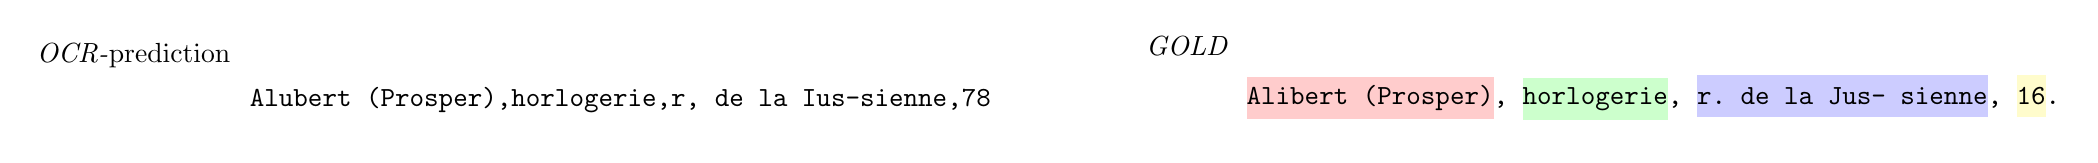
\begin{tikzpicture}
    \tikzset{alignment/.style={
        matrix of nodes, nodes={font=\tt, inner sep=0pt, minimum height=15pt}, column sep=0
      },
      taggedalignment/.style={alignment,
        column 1/.style={nodes={fill=red!20}},
        column 3/.style={nodes={fill=green!20}},
        column 5/.style={nodes={fill=blue!20}},
        column 7/.style={nodes={fill=yellow!20}},
      }
    }
  
    \node (A) { \verb|Alubert (Prosper),horlogerie,r, de la Ius-sienne,78| };
  
    \matrix[taggedalignment] (B) [right=3cm of A]
    {
      Alibert (Prosper)&,~ &horlogerie&,~ &r.~de la Jus- sienne&,~ &16&.\\
    };

    \node [above left=0cm of A, font=\it] {OCR-\emph{prediction}};
    \node [above left=0cm of B, font=\it] {GOLD};
  
  \end{tikzpicture}





  \begin{tikzpicture}
    \tikzset{alignment/.style={
        matrix of nodes, nodes={font=\tt, inner sep=0pt, minimum height=15pt}, column sep=0
      },
      taggedalignment/.style={alignment,
        column 1/.style={nodes={fill=red!20}},
        column 3/.style={nodes={fill=green!20}},
        column 5/.style={nodes={fill=blue!20}},
        column 7/.style={nodes={fill=yellow!20}},
      }
    }
  
    \node (A) { \verb|Alubert (Prosper),horlogerie,r, de la Ius-sienne,78| };
  
    \matrix[taggedalignment] (B) [right=3cm of A]
    {
      Alibert (Prosper)&,~ &horlogerie&,~ &r.~de la Jus- sienne&,~ &16&.\\
    };
  
    \matrix[alignment, row 2/.style={nodes={fill=none, gray!20}}] (C) [below=1.5cm of A]
    {
      Alibert (Prosper)&,~ &horlogerie&,~ &r.~de la Jus- sienne&,~ &16&.\\
      {||❌||||||||||||||}&{|❌}&{||||||||||}&{|❌}&{|❌❌||||||❌|||❌||||||}&{|❌}&{❌❌}&{❌}\\
      Alubert (Prosper)&,⎵ &horlogerie&,⎵  &r, de la Ius-⎵sienne&,7&8⎵ & ⎵\\
    };
  
  
    % \matrix[taggedalignment, row 2/.style={nodes={fill=none, gray!20}}] (D) at ($ (C.east)!(B)!(C.west) $)
    % {
    %   Alibert (Prosper)&,~ &horlogerie&,~ &r.~de la Jus- sienne&,~ &16&.\\
    %   {||❌||||||||||||||}&{|❌}&{||||||||||}&{|❌}&{|❌❌||||||❌|||❌||||||}&{|❌}&{❌❌}&{❌}\\
    %   Alubert (Prosper)&,⎵ &horlogerie&,⎵  &r, de la Ius-⎵sienne&,7&8⎵ & ⎵\\
    % };
  
  
    % \matrix[taggedalignment] (E1) [below=of D]
    % {
    %   Alubert (Prosper)&,⎵ &horlogerie&,⎵  &r, de la Ius-⎵sienne&,7&8⎵ & ⎵\\
    % };
  
    % \matrix[taggedalignment] (E2) [below=of E1.west, anchor=west]
    % {
    %   & Alubert (Prosper),⎵ &horlogerie&,⎵  &r, de la Ius-⎵sienne&,&78&⎵⎵\\
    % };
  
  
  
    \node [above left=0cm of A, font=\it] {OCR-\emph{prediction}};
    \node [above left=0cm of B, font=\it] {GOLD};
  
    \draw[-latex] (A.west) -- ++ (-1,0) |- (C-3-1) node[pos=0.25,left] { Alignment };
  
    % \draw[-latex] (B) -- (D) node[midway,right] { Tag projection };
    \draw[-latex] (B.west) -- ++ (-1,0) |- (C-1-8);
    % \draw[-latex] (C) -- (D);
  
  
    % \draw[-latex] (C.south) -- ++(0,-1) node[midway,right,font=\small] {OCR Q.A.} node[below] {CER = 24\%};
    % \draw[-latex] (D.south) -- ++(0,-1) node[midway,right,font=\small] {NER-\emph{target}};
    % \draw[-latex] (C.south east) |- (E2) node[pos=0.75,below, font=\it] {NER-\emph{prediction}};
    % \draw[-latex] (E2.south) -- ++(0,-1) node[midway,right,font=\small] {NER Q.A.}
    % node[below] {Precision = 66\%, Recall = 50\%, F-score = 0.4};
  \end{tikzpicture}



  \begin{tikzpicture}
    \tikzset{alignment/.style={
        matrix of nodes, nodes={font=\tt, inner sep=0pt, minimum height=15pt}, column sep=0
      },
      taggedalignment/.style={alignment,
        column 1/.style={nodes={fill=red!20}},
        column 3/.style={nodes={fill=green!20}},
        column 5/.style={nodes={fill=blue!20}},
        column 7/.style={nodes={fill=yellow!20}},
      }
    }
  
    \node (A) { \verb|Alubert (Prosper),horlogerie,r, de la Ius-sienne,78| };
  
    \matrix[taggedalignment] (B) [right=3cm of A]
    {
      Alibert (Prosper)&,~ &horlogerie&,~ &r.~de la Jus- sienne&,~ &16&.\\
    };
  
    \matrix[alignment, row 2/.style={nodes={fill=none, gray!20}}] (C) [below=1.5cm of A]
    {
      Alibert (Prosper)&,~ &horlogerie&,~ &r.~de la Jus- sienne&,~ &16&.\\
      {||❌||||||||||||||}&{|❌}&{||||||||||}&{|❌}&{|❌❌||||||❌|||❌||||||}&{|❌}&{❌❌}&{❌}\\
      Alubert (Prosper)&,⎵ &horlogerie&,⎵  &r, de la Ius-⎵sienne&,7&8⎵ & ⎵\\
    };
  
  
    % \matrix[taggedalignment, row 2/.style={nodes={fill=none, gray!20}}] (D) at ($ (C.east)!(B)!(C.west) $)
    % {
    %   Alibert (Prosper)&,~ &horlogerie&,~ &r.~de la Jus- sienne&,~ &16&.\\
    %   {||❌||||||||||||||}&{|❌}&{||||||||||}&{|❌}&{|❌❌||||||❌|||❌||||||}&{|❌}&{❌❌}&{❌}\\
    %   Alubert (Prosper)&,⎵ &horlogerie&,⎵  &r, de la Ius-⎵sienne&,7&8⎵ & ⎵\\
    % };
  
  
    % \matrix[taggedalignment] (E1) [below=of D]
    % {
    %   Alubert (Prosper)&,⎵ &horlogerie&,⎵  &r, de la Ius-⎵sienne&,7&8⎵ & ⎵\\
    % };
  
    % \matrix[taggedalignment] (E2) [below=of E1.west, anchor=west]
    % {
    %   & Alubert (Prosper),⎵ &horlogerie&,⎵  &r, de la Ius-⎵sienne&,&78&⎵⎵\\
    % };
  
  
  
    \node [above left=0cm of A, font=\it] {OCR-\emph{prediction}};
    \node [above left=0cm of B, font=\it] {GOLD};
  
    \draw[-latex] (A.west) -- ++ (-1,0) |- (C-3-1) node[pos=0.25,left] { Alignment };
  
    % \draw[-latex] (B) -- (D) node[midway,right] { Tag projection };
    \draw[-latex] (B.west) -- ++ (-1,0) |- (C-1-8);
    % \draw[-latex] (C) -- (D);
  
  
    \draw[-latex] (C.south) -- ++(0,-1) node[midway,right,font=\small] {OCR Q.A.} node[below] {CER = 24\%};
    % \draw[-latex] (D.south) -- ++(0,-1) node[midway,right,font=\small] {NER-\emph{target}};
    % \draw[-latex] (C.south east) |- (E2) node[pos=0.75,below, font=\it] {NER-\emph{prediction}};
    % \draw[-latex] (E2.south) -- ++(0,-1) node[midway,right,font=\small] {NER Q.A.}
    % node[below] {Precision = 66\%, Recall = 50\%, F-score = 0.4};
  \end{tikzpicture}


  \begin{tikzpicture}
    \tikzset{alignment/.style={
        matrix of nodes, nodes={font=\tt, inner sep=0pt, minimum height=15pt}, column sep=0
      },
      taggedalignment/.style={alignment,
        column 1/.style={nodes={fill=red!20}},
        column 3/.style={nodes={fill=green!20}},
        column 5/.style={nodes={fill=blue!20}},
        column 7/.style={nodes={fill=yellow!20}},
      }
    }
  
    \node (A) { \verb|Alubert (Prosper),horlogerie,r, de la Ius-sienne,78| };
  
    \matrix[taggedalignment] (B) [right=3cm of A]
    {
      Alibert (Prosper)&,~ &horlogerie&,~ &r.~de la Jus- sienne&,~ &16&.\\
    };
  
    \matrix[alignment, row 2/.style={nodes={fill=none, gray!20}}] (C) [below=1.5cm of A]
    {
      Alibert (Prosper)&,~ &horlogerie&,~ &r.~de la Jus- sienne&,~ &16&.\\
      {||❌||||||||||||||}&{|❌}&{||||||||||}&{|❌}&{|❌❌||||||❌|||❌||||||}&{|❌}&{❌❌}&{❌}\\
      Alubert (Prosper)&,⎵ &horlogerie&,⎵  &r, de la Ius-⎵sienne&,7&8⎵ & ⎵\\
    };
  
  
    \matrix[taggedalignment, row 2/.style={nodes={fill=none, gray!20}}] (D) at ($ (C.east)!(B)!(C.west) $)
    {
      Alibert (Prosper)&,~ &horlogerie&,~ &r.~de la Jus- sienne&,~ &16&.\\
      {||❌||||||||||||||}&{|❌}&{||||||||||}&{|❌}&{|❌❌||||||❌|||❌||||||}&{|❌}&{❌❌}&{❌}\\
      Alubert (Prosper)&,⎵ &horlogerie&,⎵  &r, de la Ius-⎵sienne&,7&8⎵ & ⎵\\
    };
  
  
    % \matrix[taggedalignment] (E1) [below=of D]
    % {
    %   Alubert (Prosper)&,⎵ &horlogerie&,⎵  &r, de la Ius-⎵sienne&,7&8⎵ & ⎵\\
    % };
  
    % \matrix[taggedalignment] (E2) [below=of E1.west, anchor=west]
    % {
    %   & Alubert (Prosper),⎵ &horlogerie&,⎵  &r, de la Ius-⎵sienne&,&78&⎵⎵\\
    % };
  
  
  
    \node [above left=0cm of A, font=\it] {OCR-\emph{prediction}};
    \node [above left=0cm of B, font=\it] {GOLD};
  
    \draw[-latex] (A.west) -- ++ (-1,0) |- (C-3-1) node[pos=0.25,left] { Alignment };
  
    \draw[-latex] (B) -- (D) node[midway,right] { Tag projection };
    \draw[-latex] (B.west) -- ++ (-1,0) |- (C-1-8);
    \draw[-latex] (C) -- (D);
  
  
    \draw[-latex] (C.south) -- ++(0,-1) node[midway,right,font=\small] {OCR Q.A.} node[below] {CER = 24\%};
    % \draw[-latex] (D.south) -- ++(0,-1) node[midway,right,font=\small] {NER-\emph{target}};
    % \draw[-latex] (C.south east) |- (E2) node[pos=0.75,below, font=\it] {NER-\emph{prediction}};
    % \draw[-latex] (E2.south) -- ++(0,-1) node[midway,right,font=\small] {NER Q.A.}
    % node[below] {Precision = 66\%, Recall = 50\%, F-score = 0.4};
  \end{tikzpicture}



  \begin{tikzpicture}
    \tikzset{alignment/.style={
        matrix of nodes, nodes={font=\tt, inner sep=0pt, minimum height=15pt}, column sep=0
      },
      taggedalignment/.style={alignment,
        column 1/.style={nodes={fill=red!20}},
        column 3/.style={nodes={fill=green!20}},
        column 5/.style={nodes={fill=blue!20}},
        column 7/.style={nodes={fill=yellow!20}},
      }
    }
  
    \node (A) { \verb|Alubert (Prosper),horlogerie,r, de la Ius-sienne,78| };
  
    \matrix[taggedalignment] (B) [right=3cm of A]
    {
      Alibert (Prosper)&,~ &horlogerie&,~ &r.~de la Jus- sienne&,~ &16&.\\
    };
  
    \matrix[alignment, row 2/.style={nodes={fill=none, gray!20}}] (C) [below=1.5cm of A]
    {
      Alibert (Prosper)&,~ &horlogerie&,~ &r.~de la Jus- sienne&,~ &16&.\\
      {||❌||||||||||||||}&{|❌}&{||||||||||}&{|❌}&{|❌❌||||||❌|||❌||||||}&{|❌}&{❌❌}&{❌}\\
      Alubert (Prosper)&,⎵ &horlogerie&,⎵  &r, de la Ius-⎵sienne&,7&8⎵ & ⎵\\
    };
  
  
    \matrix[taggedalignment, row 2/.style={nodes={fill=none, gray!20}}] (D) at ($ (C.east)!(B)!(C.west) $)
    {
      Alibert (Prosper)&,~ &horlogerie&,~ &r.~de la Jus- sienne&,~ &16&.\\
      {||❌||||||||||||||}&{|❌}&{||||||||||}&{|❌}&{|❌❌||||||❌|||❌||||||}&{|❌}&{❌❌}&{❌}\\
      Alubert (Prosper)&,⎵ &horlogerie&,⎵  &r, de la Ius-⎵sienne&,7&8⎵ & ⎵\\
    };
  
  
    \matrix[taggedalignment] (E1) [below=of D]
    {
      Alubert (Prosper)&,⎵ &horlogerie&,⎵  &r, de la Ius-⎵sienne&,7&8⎵ & ⎵\\
    };
  
    % \matrix[taggedalignment] (E2) [below=of E1.west, anchor=west]
    % {
    %   & Alubert (Prosper),⎵ &horlogerie&,⎵  &r, de la Ius-⎵sienne&,&78&⎵⎵\\
    % };
  
  
  
    \node [above left=0cm of A, font=\it] {OCR-\emph{prediction}};
    \node [above left=0cm of B, font=\it] {GOLD};
  
    \draw[-latex] (A.west) -- ++ (-1,0) |- (C-3-1) node[pos=0.25,left] { Alignment };
  
    \draw[-latex] (B) -- (D) node[midway,right] { Tag projection };
    \draw[-latex] (B.west) -- ++ (-1,0) |- (C-1-8);
    \draw[-latex] (C) -- (D);
  
  
    \draw[-latex] (C.south) -- ++(0,-1) node[midway,right,font=\small] {OCR Q.A.} node[below] {CER = 24\%};
    \draw[-latex] (D.south) -- ++(0,-1) node[midway,right,font=\small] {NER-\emph{target}};
    % \draw[-latex] (C.south east) |- (E2) node[pos=0.75,below, font=\it] {NER-\emph{prediction}};
    % \draw[-latex] (E2.south) -- ++(0,-1) node[midway,right,font=\small] {NER Q.A.}
    % node[below] {Precision = 66\%, Recall = 50\%, F-score = 0.4};
  \end{tikzpicture}







\begin{tikzpicture}
  \tikzset{alignment/.style={
      matrix of nodes, nodes={font=\tt, inner sep=0pt, minimum height=15pt}, column sep=0
    },
    taggedalignment/.style={alignment,
      column 1/.style={nodes={fill=red!20}},
      column 3/.style={nodes={fill=green!20}},
      column 5/.style={nodes={fill=blue!20}},
      column 7/.style={nodes={fill=yellow!20}},
    }
  }

  \node (A) { \verb|Alubert (Prosper),horlogerie,r, de la Ius-sienne,78| };

  \matrix[taggedalignment] (B) [right=3cm of A]
  {
    Alibert (Prosper)&,~ &horlogerie&,~ &r.~de la Jus- sienne&,~ &16&.\\
  };

  \matrix[alignment, row 2/.style={nodes={fill=none, gray!20}}] (C) [below=1.5cm of A]
  {
    Alibert (Prosper)&,~ &horlogerie&,~ &r.~de la Jus- sienne&,~ &16&.\\
    {||❌||||||||||||||}&{|❌}&{||||||||||}&{|❌}&{|❌❌||||||❌|||❌||||||}&{|❌}&{❌❌}&{❌}\\
    Alubert (Prosper)&,⎵ &horlogerie&,⎵  &r, de la Ius-⎵sienne&,7&8⎵ & ⎵\\
  };


  \matrix[taggedalignment, row 2/.style={nodes={fill=none, gray!20}}] (D) at ($ (C.east)!(B)!(C.west) $)
  {
    Alibert (Prosper)&,~ &horlogerie&,~ &r.~de la Jus- sienne&,~ &16&.\\
    {||❌||||||||||||||}&{|❌}&{||||||||||}&{|❌}&{|❌❌||||||❌|||❌||||||}&{|❌}&{❌❌}&{❌}\\
    Alubert (Prosper)&,⎵ &horlogerie&,⎵  &r, de la Ius-⎵sienne&,7&8⎵ & ⎵\\
  };


  \matrix[taggedalignment] (E1) [below=of D]
  {
    Alubert (Prosper)&,⎵ &horlogerie&,⎵  &r, de la Ius-⎵sienne&,7&8⎵ & ⎵\\
  };

  \matrix[taggedalignment] (E2) [below=of E1.west, anchor=west]
  {
    & Alubert (Prosper),⎵ &horlogerie&,⎵  &r, de la Ius-⎵sienne&,&78&⎵⎵\\
  };



  \node [above left=0cm of A, font=\it] {OCR-\emph{prediction}};
  \node [above left=0cm of B, font=\it] {GOLD};

  \draw[-latex] (A.west) -- ++ (-1,0) |- (C-3-1) node[pos=0.25,left] { Alignment };

  \draw[-latex] (B) -- (D) node[midway,right] { Tag projection };
  \draw[-latex] (B.west) -- ++ (-1,0) |- (C-1-8);
  \draw[-latex] (C) -- (D);


  \draw[-latex] (C.south) -- ++(0,-1) node[midway,right,font=\small] {OCR Q.A.} node[below] {CER = 24\%};
  \draw[-latex] (D.south) -- ++(0,-1) node[midway,right,font=\small] {NER-\emph{target}};
  \draw[-latex] (C.south east) |- (E2) node[pos=0.75,below, font=\it] {NER-\emph{prediction}};
  \draw[-latex] (E2.south) -- ++(0,-1) node[midway,right,font=\small] {NER Q.A.}
  node[below] {Precision = 66\%, Recall = 50\%, F-score = 0.4};
\end{tikzpicture}



\end{document}